\newpage
\section{特征选择与稀疏学习}
特征: 描述物体的属性

特征的分类:
\begin{itemize}
    \item 相关特征: 对当前学习任务有用的属性
    \item 无关特征: 与当前学习任务无关的属性
    \item 冗余特征${}^*$: 其所包含信息能由其他特征推演出来
\end{itemize}

特征选择: 从给定的特征集合中选出任务相关特征子集, 必须确保不丢失重要特征. 
\subsection{子集搜索与评价}
用贪心策略选择包含重要信息的特征子集
\begin{itemize}
    \item 前向搜索:逐渐增加相关特征
    \item 后向搜索:从完整的特征集合开始,逐渐减少特征
    \item 双向搜索:每一轮逐渐增加相关特征,同时减少无关特征
\end{itemize}

特征子集确定了对数据集的一个划分, 每个划分区域对应着特征子集的某种取值. 样本标记对应着对数据集的真实划分. 通过估算这两个划分的差异,就能对特征子集进行评价;与样本标记对应的划分的差异越小,则说明当前特征子集越好. 

比如用信息熵进行子集评价. 

\subsection{过滤式选择}
先用特征选择过程过滤原始数据,再用过滤后的特征来训练模型;特征选择过程与后续学习器无关. 

Relief (Relevant Features) 方法
\subsection{包裹式选择}
包裹式选择直接把最终将要使用的学习器的性能作为特征子集的评价准则. 


LVW(Las Vegas Wrapper) 在拉斯维加斯方法框架下使用随机策略来进行子集搜索,并以最终分类器的误差作为特征子集评价准则
\subsection{嵌入式选择与\texorpdfstring{$L_1$}.  正则化}
嵌入式特征选择是将特征选择过程与学习器训练过程融为一体,两者在同一个优化过程中完成,在学习器训练过程中自动地进行特征选择


{$L_1$}正则化: 采用$L_1$范数时交点常出现在坐标轴上,即容易产生值为0的稀疏解. 

\begin{figure}[!htb]
    \centering
    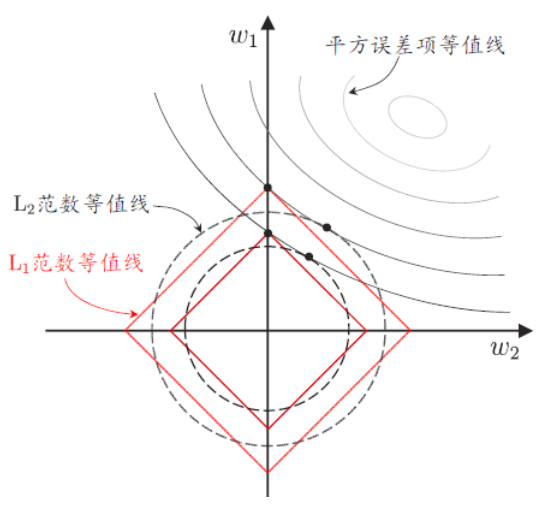
\includegraphics[width=0.309\textwidth]{pic/L1正则化.png}
    \caption{{$L_1$}正则化}
\end{figure}


\subsection{稀疏表示与字典学习}
\subsubsection{稀疏表示}
将数据集考虑成一个矩阵,每行对应一个样本,每列对应一个特征. 矩阵中有很多零元素,且非整行整列出现. 

稀疏表达的优势:
\begin{itemize}
    \item 文本数据线性可分
    \item 存储高效
\end{itemize}

\subsubsection{字典学习}
为普通稠密表达的样本找到合适的字典,将样本转化为
稀疏表示,这一过程称为字典学习


\subsection{压缩感知}
利用部分数据恢复全部数据